%
% $RCSfile: specification_language.tex,v $
%
% Copyright (C) 2002-2008. Christian Heller.
%
% Permission is granted to copy, distribute and/or modify this document
% under the terms of the GNU Free Documentation License, Version 1.1 or
% any later version published by the Free Software Foundation; with no
% Invariant Sections, with no Front-Cover Texts and with no Back-Cover
% Texts. A copy of the license is included in the section entitled
% "GNU Free Documentation License".
%
% http://www.cybop.net
% - Cybernetics Oriented Programming -
%
% http://www.resmedicinae.org
% - Information in Medicine -
%
% Version: $Revision: 1.1 $ $Date: 2008-08-19 20:41:09 $ $Author: christian $
% Authors: Christian Heller <christian.heller@tuxtax.de>
%

\subsection{Specification Language}
\label{specification_language_heading}
\index{Specification Language}
\index{Unified Modeling Language}
\index{UML}
\index{Feature Model}
\index{Z Specification Language}
\index{B Specification Language}
\index{Vienna Development Method - Specification Language}
\index{VDM-SL}
\index{Specification and Description Language}
\index{SDL}
\index{Extended Meta Language}
\index{Extended ML}

A \emph{Specification Language}, after \cite{wikipedia}, were a formal language
used during system analysis and design, as opposed to a \emph{Programming Language},
which were a mostly directly executable formal language used to implement a system.
As its name already indicates, a specification language describes systems at a much
higher abstract level than a programming language does. But that also means that it:
\textit{must be subject to a process of refinement (the filling-in of implementation
detail), before it can actually be implemented}, as \cite{wikipedia} writes.

Many kinds of specification languages exist. Being a de facto standard, only
the first two of those representatives listed following are introduced in
slightly more detail below:

\begin{itemize}
    \item[-] \emph{Unified Modeling Language} (UML) \cite{uml}
    \item[-] \emph{Feature Model} \cite{foda}
    \item[-] \emph{Z Specification Language} \cite{zspeclang} and
        \emph{B Specification Language} \cite{zb2005}
    \item[-] \emph{Vienna Development Method - Specification Language} (VDM-SL) \cite{vdmsl}
    \item[-] \emph{Specification and Description Language} (SDL) \cite{sdl}
    \item[-] \emph{Extended Meta Language} (Extended ML) \cite{extendedml}
\end{itemize}

%
% $RCSfile: unified_modeling_language.tex,v $
%
% Copyright (C) 2002-2008. Christian Heller.
%
% Permission is granted to copy, distribute and/or modify this document
% under the terms of the GNU Free Documentation License, Version 1.1 or
% any later version published by the Free Software Foundation; with no
% Invariant Sections, with no Front-Cover Texts and with no Back-Cover
% Texts. A copy of the license is included in the section entitled
% "GNU Free Documentation License".
%
% http://www.cybop.net
% - Cybernetics Oriented Programming -
%
% http://www.resmedicinae.org
% - Information in Medicine -
%
% Version: $Revision: 1.1 $ $Date: 2008-08-19 20:41:09 $ $Author: christian $
% Authors: Christian Heller <christian.heller@tuxtax.de>
%

\subsubsection{Unified Modeling Language}
\label{unified_modeling_language_heading}
\index{Unified Modeling Language}
\index{UML}
\index{Class Diagram}
\index{Activity Diagram}
\index{Sequence Diagram}
\index{Use Case Diagram}
\index{State Machine Diagram}
\index{State Chart Diagram}
\index{Component Diagram}
\index{Deployment Diagram}
\index{Object Diagram}
\index{Instance Diagram}
\index{Package Diagram}
\index{Communication Diagram}
\index{Collaboration Diagram}
\index{Composite Structure Diagram}
\index{Interaction Overview Diagram}
\index{Timing Diagram}
\index{UML Diagram Type}
\index{Object Constraint Language}
\index{OCL}
\index{Structure Diagram}
\index{Behaviour Diagram}
\index{Interaction Diagram}
\index{Functional Model}
\index{Object Model}
\index{Dynamic Model}
\index{UML Tool}
\index{Computer Aided Software Engineering Tool}
\index{CASE Tool}
\index{Object Process Diagram}
\index{OPD}
\index{Entity Relationship Diagram}
\index{ERD}

Meanwhile, the probably most famous modelling- and specification language is
the \emph{Unified Modeling Language} (UML) \cite{uml, booch}. It uses a
graphical notation defining a number of diagrams. UML 2.x specifications
\cite{uml} extend the number of different diagram types from 9 (UML 1.x) to 13.
A good overview is given by Ambler in \cite{ambler2005}, which table
\ref{diagrams_table} reproduces in adapted form, showing only \emph{some}
diagram elements. The column \emph{Importance} contains a certainly subjective
recommendation of Ambler, indicating the \emph{Learning Priority} the single
diagram types have in his opinion (which the author of this work supports).

\begin{table}[ht]
    \begin{center}
        \begin{footnotesize}
        \begin{tabular}{| p{35mm} | p{55mm} | p{15mm} |}
            \hline
            \textbf{Diagram} & \textbf{Elements} & \textbf{Importance}\\
            \hline
            Class (CsD) & Class, Inheritance, Association & High\\
            \hline
            Activity (AD) & Activity, Flow, Fork/ Join, Condition, Decision/ Merge & High\\
            \hline
            Sequence (SD) & Object, Lifeline, Activation Box (Method-Invocation Box), Message & High\\
            \hline
            Use Case (UCD) & Use Case, Actor, Association & Medium\\
            \hline
            State Machine (SMD), formerly State Chart Diagram & State, Transition & Medium\\
            \hline
            Component (CmD) & Component, Interface, Dependency & Medium\\
            \hline
            Deployment (DD) & Node, Connection & Medium\\
            \hline
            Object (ObD), also referred to as Instance Diagram & Object, Relationship & Low\\
            \hline
            Package (PD) & Package, Dependency & Low\\
            \hline
            Communication (CoD), formerly Collaboration Diagram & Object, Association & Low\\
            \hline
            Composite Structure (CSD) & Collaboration, Object, Role & Low\\
            \hline
            Interaction Overview (IOD) & Interaction Frame, Interaction Occurrence Frame & Low\\
            \hline
            Timing (TiD) & Object, Lifeline, State, Timing Constraint & Low\\
            \hline
        \end{tabular}
        \end{footnotesize}
        \caption{UML 2.x Diagram Types \cite{ambler2005}}
        \label{diagrams_table}
    \end{center}
\end{table}

One extension to the UML that is now also part of the corresponding de-facto
standard, is the \emph{Object Constraint Language} (OCL). Being a declarative
language, it describes rules applying to UML models, in a precise text format.
This is because not all rules can be expressed by diagrammatic notation
\cite{wikipedia}. The range of possible rules comprises constraints like pre-
and post-conditions or object query expressions. \cite{ocl}

A common classification distinguishes UML diagrams as follows \cite{ambler2005}:

\begin{enumerate}
    \item \emph{Structure:} CsD, CmD, CSD, DD, ObD, PD
    \item \emph{Behaviour:} AD, SMD, UCD
    \item \emph{Interaction:} CoD, IOD, SD, TiD
\end{enumerate}

Others share the information represented by the diagrams according to an
underlying, independently existing model \cite{wikipedia}:

\begin{itemize}
    \item[-] \emph{Functional Model} (UCD): Functionality of the system from
        the user's point of view
    \item[-] \emph{Object Model} (CsD): Structure and substructure of the
        system using objects, attributes, operations, and associations
    \item[-] \emph{Dynamic Model} (AD, SD, SCD): Internal behaviour of the
        system
\end{itemize}

A program working with UML diagrams is called \emph{UML Tool}, or more exactly
\emph{Computer Aided Software Engineering} (CASE) tool. Many of these programs
have developed and matured, over the past decade of years. Besides the standard
UML diagram types, they offer source code parsing and -generation,
documentation creation and more. Some tools introduced their own extensions to
the UML de-facto standard, for example: \emph{Object Process Diagram} (OPD)
\cite{burkhardt} and \emph{Entity Relationship Diagram} (ERD) \cite{otw}. The
description of a hypothetic design tool suggested for the language being
introduced in chapter \ref{cybernetics_oriented_language_heading} will refer
back to the UML diagrams as mentioned in this section, and suggest a different
way to categorise them. Further, chapter \ref{cybernetics_oriented_language_heading}
will try to define four diagram types to be used in conjunction with the
language described in it.

%
% $RCSfile: feature_model.tex,v $
%
% Copyright (C) 2002-2008. Christian Heller.
%
% Permission is granted to copy, distribute and/or modify this document
% under the terms of the GNU Free Documentation License, Version 1.1 or
% any later version published by the Free Software Foundation; with no
% Invariant Sections, with no Front-Cover Texts and with no Back-Cover
% Texts. A copy of the license is included in the section entitled
% "GNU Free Documentation License".
%
% http://www.cybop.net
% - Cybernetics Oriented Programming -
%
% http://www.resmedicinae.org
% - Information in Medicine -
%
% Version: $Revision: 1.1 $ $Date: 2008-08-19 20:41:06 $ $Author: christian $
% Authors: Christian Heller <christian.heller@tuxtax.de>
%

\subsubsection{Feature Model}
\label{feature_model_heading}
\index{Feature Model}
\index{Feature Modelling}
\index{System Family}
\index{Software Product Line}
\index{Feature Driven Design}
\index{Software Engineering Process}
\index{SEP}
\index{Feature Oriented Domain Analysis}
\index{FODA}
\index{Traceability}

Czarnecki \cite{czarnecki} sees \emph{Feature Modelling}, a technique for
analysing and capturing \emph{common} and \emph{variable} features of a family
of systems as well as their inter-dependencies in form of a \emph{Feature Model},
as the main contribution of domain engineering to OOA/ OOD methods. The
\emph{System Families}, also called \emph{Software Product Lines}, whose
development feature models shall support, are described by Kai Boellert
\cite{boellert} as \textit{group of software systems that are developed from a
common set of reusable components}. Czarnecki writes:

\begin{quote}
    \emph{Feature Models} represent the configurability aspect of reusable
    software at an abstract level, i.e. without committing to any particular
    implementation technique such as inheritance, aggregation, or parameterized
    classes. Developers construct the initial models of the reusable software
    in the form of feature models and use them to \emph{guide} the design and
    implementation (also called \emph{Feature-driven Design}). To a reuser, on
    the other hand, feature models represent an \emph{overview} of the
    functionality of the reusable software and a guide to \emph{configuring} it
    for a specific usage context.
\end{quote}

\begin{figure}[ht]
    \begin{center}
        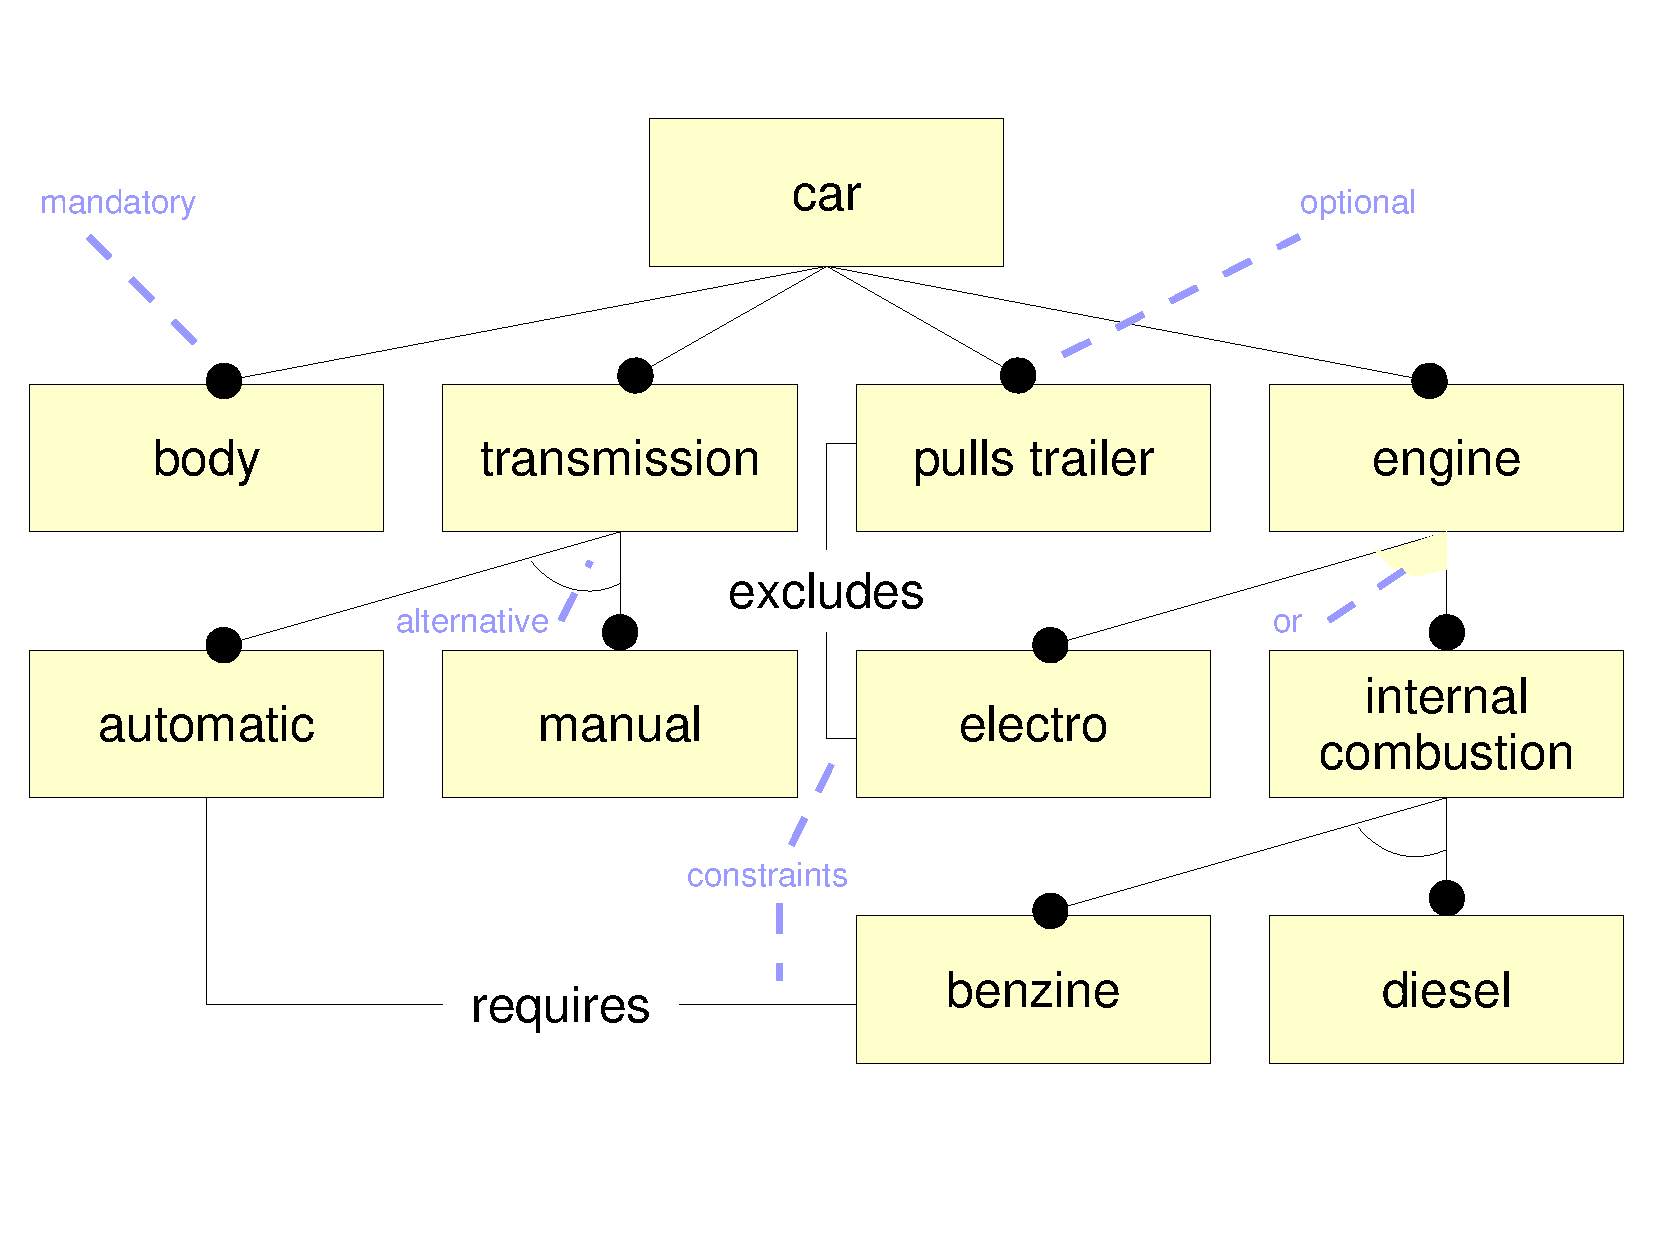
\includegraphics[scale=0.3,angle=-90]{graphic/feature.pdf}
        \caption{Classical Feature Model Diagram of a Car (based on \cite{pashov})}
        \label{feature_figure}
    \end{center}
\end{figure}

In other words, a feature model (figure \ref{feature_figure}) is an additional
form of abstraction within a \emph{Software Engineering Process} (SEP), placed
between analysis- and design models. The properties contained in a feature model
are structured hierarchically. In the \emph{Feature Oriented Domain Analysis}
(FODA) \cite{foda}, a feature model distinguishes three kinds of features:
\emph{Context}, \emph{Representation}, \emph{Operational}. Detlef Streitferdt
\cite{streitferdt200412} defines five feature types:

\begin{enumerate}
    \item \emph{Functional:} used by customer to compose a system
    \item \emph{Interface:} describe required and provided component interfaces
    \item \emph{Parameter:} used to configure functional features
    \item \emph{Structural:} relevant for an automated choice of components
    \item \emph{Conditional:} summarise sub-features to improve readability
\end{enumerate}

Using feature models, the \emph{Traceability} between concrete requirements and
architecture components can be improved. Requirements can better be mapped to
architecture elements, so that also the \emph{Communication} between
stakeholders in the development process can profit. The big abstraction gap
(number \emph{1} in figure \ref{gaps_figure} of section
\ref{abstraction_gaps_heading}) gets split into two smaller (\emph{1a} and
\emph{1b} in figure \ref{gaps_figure}) that do not close the gap conclusively,
but make it easier to cross. The disadvantage of using feature models in a SEP,
however, is that another abstraction gap causing additional effort is created
through them.

The knowledge schema and language introduced in chapters
\ref{knowledge_schema_heading} and \ref{cybernetics_oriented_language_heading}
use a hierarchical structure comparable to the feature model. Their elements,
though, do belong to just one of two possible kinds: \emph{whole-part} model or
\emph{meta property} model. CYBOP knowledge models merge \emph{some} of the
information that would traditionally be found in feature models with that
contained in the design diagrams and might thus be able to eliminate gap 1b.
Non-functional requirements like \emph{Performance}, \emph{Scalability},
\emph{Usability} or \emph{Memory Efficiency} are \emph{not} part of a CYBOP
knowledge model, since they have nothing to do with the actual modelling of
real-world items in form of abstract concepts and belong into a corresponding
analysis- and specification document only.

